\documentclass{beamer}


\usepackage[utf8]{inputenc}
\usepackage{polski, graphicx}
\usetheme{Warsaw}

\title
{System pisania testów na platformie Android}
\subtitle{Seminarium dyplomowe}
\author{Filip Malinowski}
\subject{Seminarium}


\begin{document}

  \begin{frame}
	\titlepage
  \end{frame}

  \begin{frame}
    \frametitle{Plan prezentacji}
    \begin{itemize}
    \item Opis projektu inżynierskiego
    \item Cel projektu
    \item Dostępne narzędzia tworzenia aplikacji mobilnej
    \item Komunikacja z serwerem
    \item Dostępne aplikacje serwerowe
    \item Postęp prac
    \item Szyfrowanie plików
    \item Testy aplikacji
    \item Wygląd aplikacji
    \end{itemize}
  \end{frame}

  \begin{frame}
    \frametitle{Opis projektu inżynierskiego}
    Docelowo projekt ma zawierać:
    \begin{itemize}
    \item aplikację na systemy Android
    \item serwer do obsługi aplikacji
    \end{itemize}
    Aplikacje mają się komunikować przez Internet z serwerem oraz przesyłać do
    niego odpowiedzi studentów. Serwer ma otrzymane dane obsłużyć i przedstawić
    w formacie odpowiednim dla prowadzącego.
  \end{frame}

  \begin{frame}
    \frametitle{Cel projektu}
    Stworzenie niezawodnego systemu na platformę Android umożliwiającego pisanie testów na wykładach akademickich i zautomatyzowane zbieranie i przetwarzanie wyników testów.
  \end{frame}

  \begin{frame}
    \frametitle{Dostępne narzędzia tworzenia aplikacji mobilnej}
    Środowiska w jakich można napisać aplikację na system Android to:
    \begin{itemize}
    \item Android studio
    \item Qt (w wersji równej 5.1 lub wyższej)
    \end{itemize}
  \end{frame}

  \begin{frame}
	\frametitle{Komunikacja z serwerem}
	Protokoły komunikacyjne jakie można wykorzystać między aplikacją mobilną a serwerem:
	\begin{itemize}
		\item HTTP
		\item TCP
		\item UDP
	\end{itemize}
  \end{frame}

  \begin{frame}
    \frametitle{Dostępne aplikacje serwerowe}
    Aplikacje jakie można wykorzystać to stworzenia serwera opierającego się na protokole HTTP:\\
    \begin{itemize}
    \item Nginx
    \item OpenLiteSpeed
    \item Apache
    \end{itemize}
  \end{frame}

  \begin{frame}
    \frametitle{Postęp prac}
    \begin{itemize}
    \item Androidowa aplikacja komunikująca się z serwerem Apache
    \item Skrypt do parsowania logów jako zastępstwo dla pełnoprawnego serwera
    \item Program deszyfrujący pliki na telefonach
    \item Program tworzący plik konfiguracyjny testu
    \end{itemize}
  \end{frame}

  \begin{frame}
	\frametitle{Szyfrowanie plików}
	Odpowiedzi szyfrowane algorytmem RSA. Klucz publiczny pobierany z serwera wykorzystany przy szyfrowaniu. Ziarno (ang. salt) użyte do podniesienia stopnia zabezpieczenia zaszyfrowanych danych.
  \end{frame}

  \begin{frame}
    \frametitle{Testy aplikacji}
    \begin{itemize}
    \item Pomyślnie wykonane 7 testów 16-to pytaniowych na AiR na W-10 i tylko 1 test z problemami
    \item Pomyślnie wykonany test 64-pytaniowy na AiR na W-4
    \end{itemize}
  \end{frame}

  \begin{frame}
  	\frametitle{Widok główny}
  	\begin{center}
  		\begin{figure}[ht]
  			\centering
  			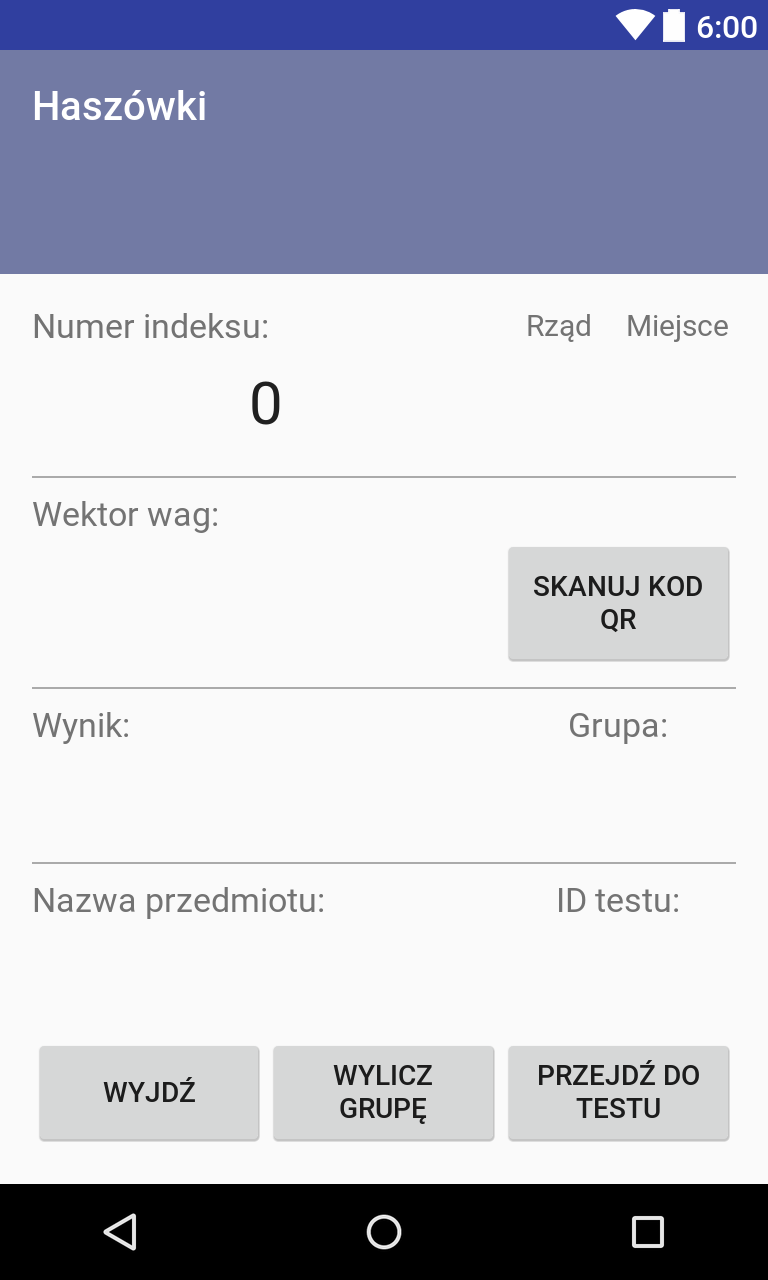
\includegraphics[scale=0.15]{layout-2016-11-29-223545.png}
  		\end{figure}
  	\end{center}
  \end{frame}

  \begin{frame}
	\frametitle{Widok ustawień}
	\begin{center}
		\begin{figure}[ht]
			\centering
			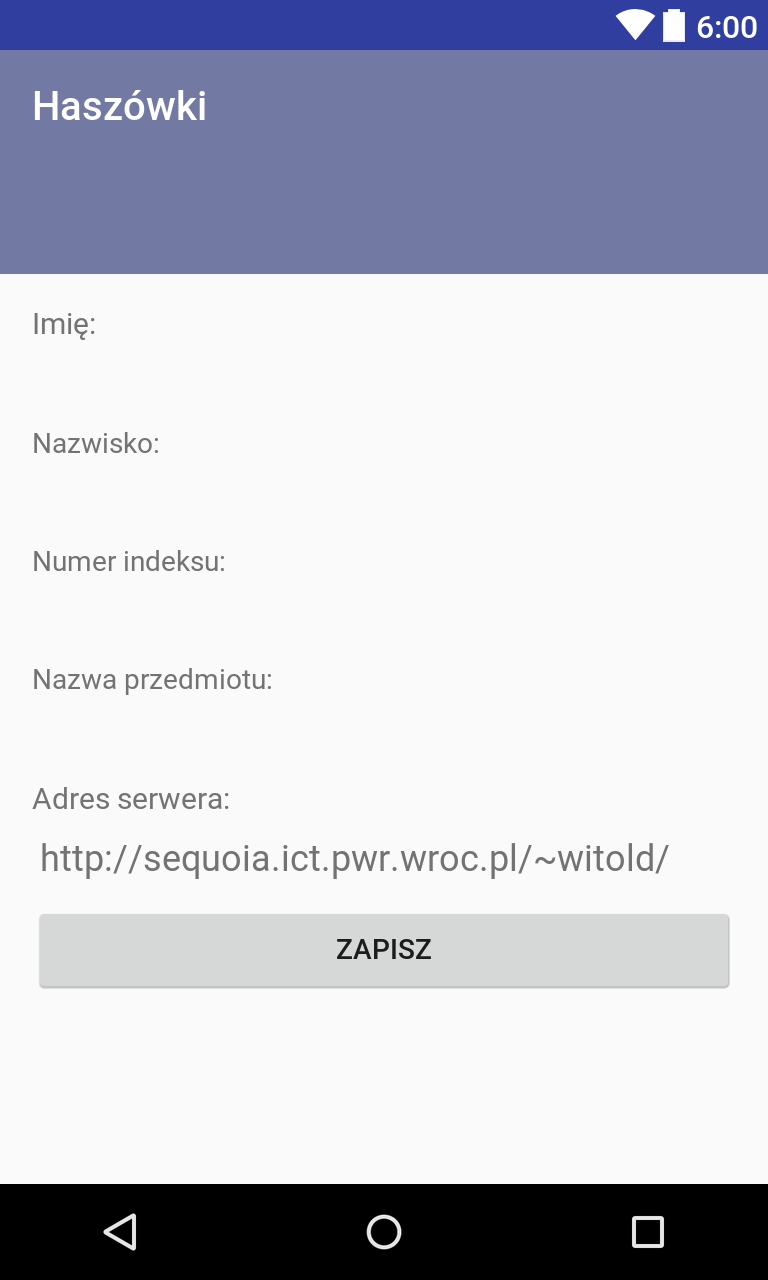
\includegraphics[scale=0.15]{layout-2016-11-29-223623.png}
		\end{figure}
	\end{center}
  \end{frame}

  \begin{frame}
	\frametitle{Widok konfiguracji testu}
	\begin{center}
		\begin{figure}[ht]
			\centering
			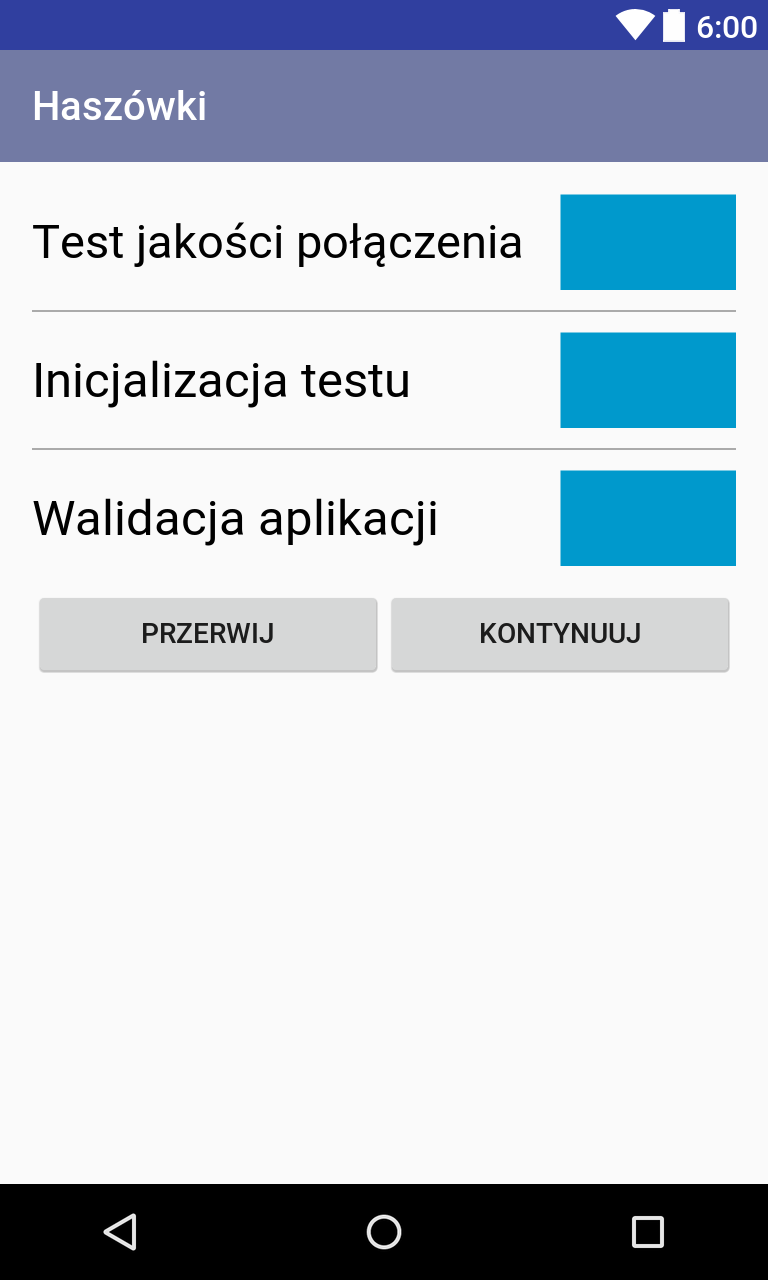
\includegraphics[scale=0.15]{layout-2016-11-29-223634.png}
		\end{figure}
	\end{center}
  \end{frame}

  \begin{frame}
	\frametitle{Widok testu}
	\begin{center}
		\begin{figure}[ht]
			\centering
			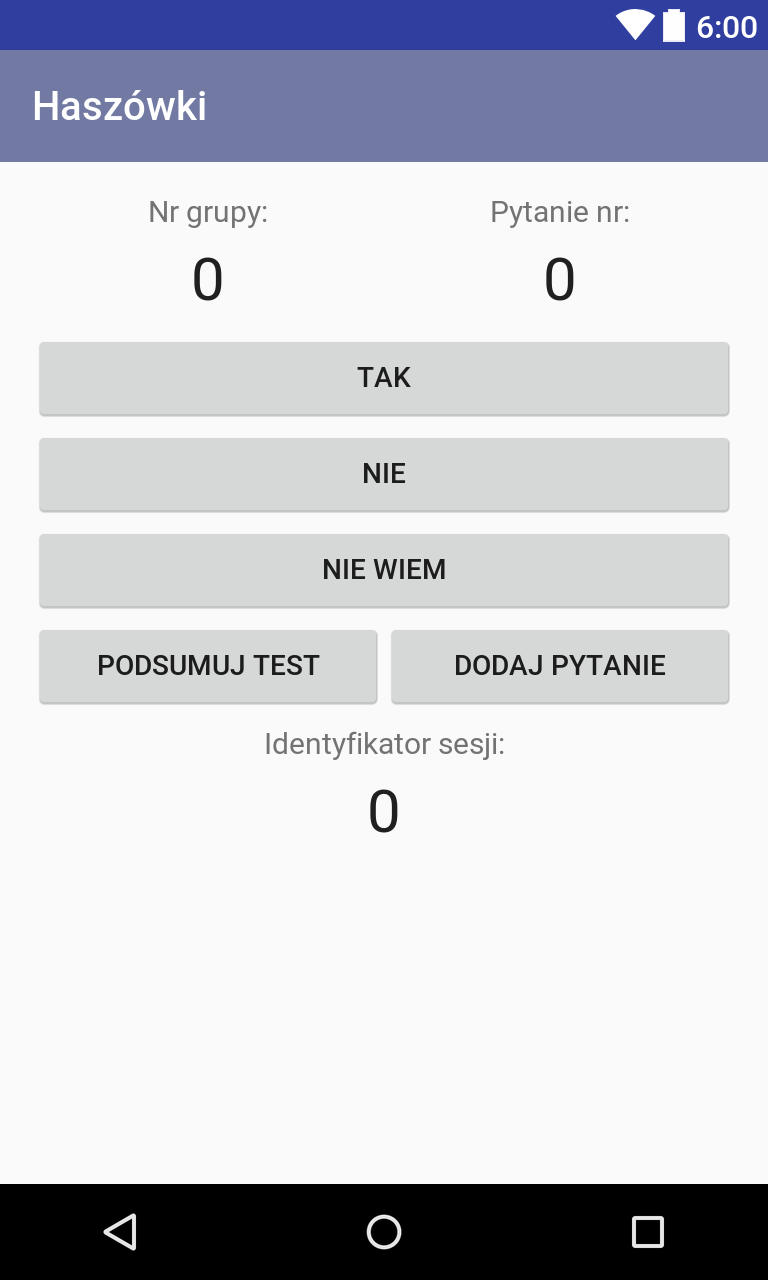
\includegraphics[scale=0.15]{layout-2016-11-29-223644.png}
		\end{figure}
	\end{center}
  \end{frame}


  \begin{frame}
	\frametitle{Widok podsumowania}
	\begin{center}
		\begin{figure}[ht]
			\centering
			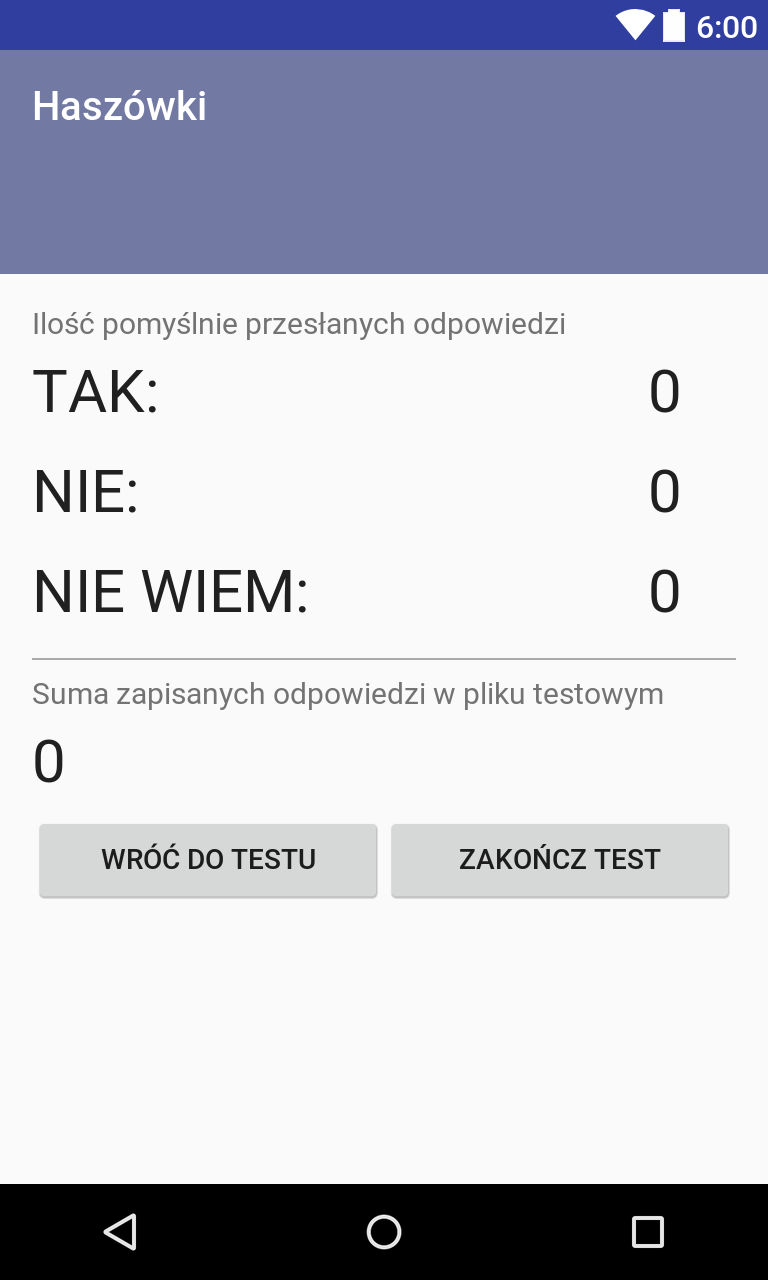
\includegraphics[scale=0.15]{layout-2016-11-29-223656.png}
		\end{figure}
	\end{center}
  \end{frame}

  \begin{frame}
  	\frametitle{Koniec}
    \begin{center}
    \Huge Dziękuję za uwagę
    \end{center}
  \end{frame}
% etc
\end{document}